
\chapter{Optical Fiber Impairments}
\label{chap:fiber_impairments}


\section{Introduction}

Propagation through an optical fiber distorts a frequency signal. Previous work described the various optical impairments in an optical fiber and their influence on a frequency signal \cite{menyukIFCS2015}. In this chapter, we summarize that work and relate it to our simulations.

The optical fiber communication system transmits information over multiple data signals separated in the frequency domain in a scheme called wavelength division multiplexing (WDM). The data signals have center frequencies that are spaced $10$--$100$ GHz apart and are on the order of $100$ THz, in agreement with the ITU standard \cite{ITU-T2012}. A frequency signal will have a smaller bandwidth than the data signals and can be included alongside the data traffic. The frequency signal's bandwidth is also small enough that we can place the frequency signal between two data signals that are centered at adjacent center frequencies, as shown in Figure~\ref{fig:system}. However, placing the frequency signal in this manner leads to nonlinear coupling between the neighboring data signals and the frequency signal and thus distortion of the frequency signal.

\begin{figure}
	\raggedright
	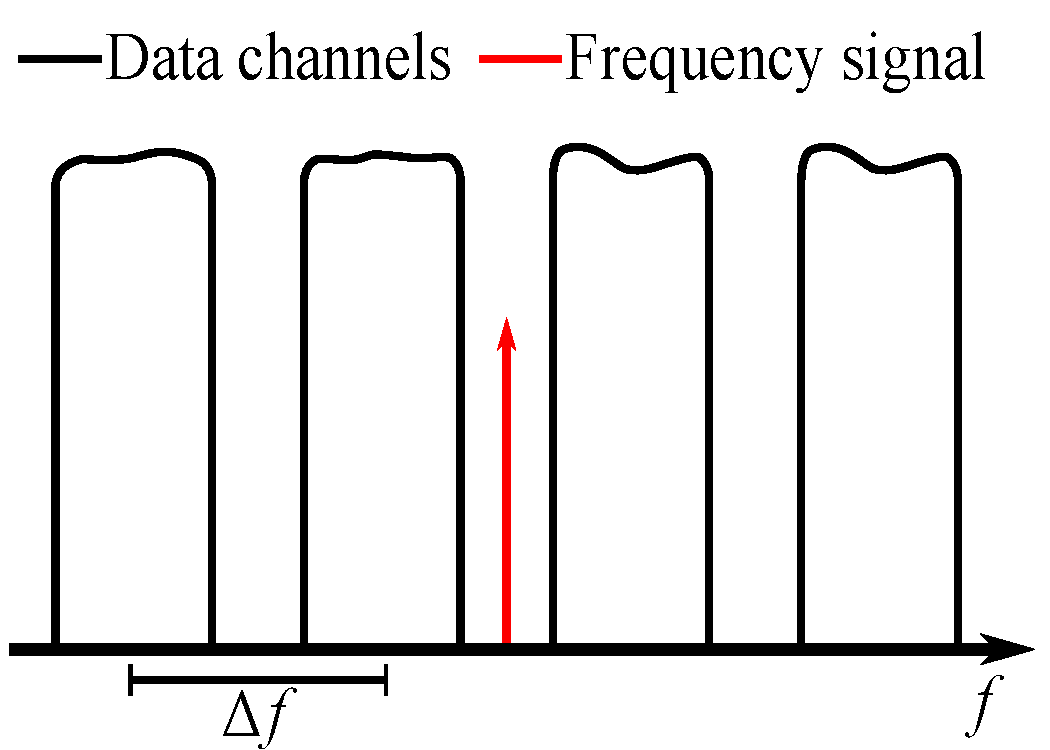
\includegraphics[scale=0.6]{img/system.pdf}
	\renewcommand{\baselinestretch}{1}
	\small\normalsize
	\caption{Desired frequency domain placement of the frequency signal.	\label{fig:system}}
\end{figure}
\renewcommand{\baselinestretch}{2}
\small\normalsize

We will study an optical fiber communication system with multiple WDM data channels centered around the wavelength $1530$ nm and with a bandwidth of $10$ GHz for each channel. The data signals are modulated as non-return-to-zero on-off-keyed (NRZ-OOK) symbols. The optical fiber is a single-mode fiber in which light propagation is impaired by second-order dispersion, the Kerr nonlinearity, and attenuation \cite{agrawal2012fiber,Agrawal2013}. Brillouin scattering, Raman scattering, and Rayleigh scattering can also impair light propagation \cite{Boyd2003}.

In this chapter, we first examine coupled propagation equations for a single data channel and a frequency signal that are separated in the frequency domain. Then, we generalize the coupled equations to account for multiple data channels and a single frequency signal. We further examine each of the impairment terms in the equations, and we will give suitable conditions under which they can be neglected when calculating the phase stability. We will then show that the impairment due to cross-phase modulation is the primary optical source of phase instability.

\section{Coupled Propagation Equations} \label{sec:cnlse}

We begin by considering the interaction of a single data channel and a frequency signal and derive their propagation equations. The small bandwidth of an optical signal compared to the central frequency in an optical fiber allows us to use a slowly varying envelope approximation for the propagation of light \cite{Agrawal2013}. If we consider the interaction of a frequency signal with a single data channel, the electric field becomes a sum of the products of a rapidly varying carrier signal and a slowly varying envelope,
%
\begin{equation}
\mathbf{E}(\mathbf{r}, t) = \frac{1}{2}\hat{\mathbf{x}}\left[ E_d\exp(-i\omega_dt) + E_f\exp(-i\omega_ft)\right] + c.c.,
\end{equation}
%
where $\hat{\mathbf{x}}$ is the direction of polarization, $\omega_j$ for $j=d,f$ are the carrier frequencies for a data channel and the frequency signal respectively, and the $E_j$ are the slowly varying time envelopes. We assume that each of the envelopes may be written as
%
\begin{equation}
E_j(\mathbf{r}, t) = F_j(x,y)u_j(z,t)\exp(i\beta_{0j}z),
\end{equation}
%
where $j=d,f$ corresponds to the appropriate envelope, $F_j(x,y)$ is the distribution of the fiber mode in the plane normal to the propagation direction, $u_j(z,t,)$ is the slowly varying amplitude, and $\beta_{0j}$ is the phase shift associated with propagation distance. Separating the propagation and transverse directions is justified by the large discrepancy in the length scales between the transverse and propagation directions \cite{Agrawal2013}. We then obtain an equation for each envelope $u_j$ in the form of coupled nonlinear Schr{\"o}dinger (NLS) equations \cite{Agrawal2013},
%
\begin{equation}
\frac{\partial u_j}{\partial z} + \beta_{1j}\frac{\partial u_j}{\partial t} + \frac{i\beta_{2j}}{2}\frac{\partial^2 u_j}{\partial t^2} + \frac{\alpha_j}{2}u_j = \frac{in_2\omega_j}{c}\left(f_{jj}|u_j|^2 + 2f_{jk}|u_k|^2\right)u_j,
\end{equation}
%
where $j\neq k$, $j,k = d,f$ for the two envelopes, $\beta_{1j} = 1/v_{gj}$ is the corresponding inverse group velocity, $\beta_{2j}$ is the corresponding group velocity dispersion, and $\alpha_j$ is the attenuation. The terms on the right-hand side represent the nonlinear impairment, $n_2$ is the nonlinear Kerr parameter, and the $f_{jk}$ are the overlap integrals defined as
%
\begin{equation}
f_{jk} = \frac{\int_{-\infty}^{\infty}\int_{-\infty}^{\infty} |F_j(x,y)|^2|F_k(x,y)|^2dxdy }{\int_{-\infty}^{\infty}\int_{-\infty}^{\infty} |F_j(x,y)|^2dxdy\int_{-\infty}^{\infty}\int_{-\infty}^{\infty}|F_k(x,y)|^2dxdy}.
\end{equation}
%
Since the system that we consider uses conventional single-mode fibers, the overlap integrals $f_{jk}$ are all nearly the same. We neglect the differences and write the integrals as $f_{dd} = f_{df} = f_{ff} = 1/A_{\text{eff}}$. This approximation allows us to simplify the right-hand side further by introducing the nonlinear parameter $\gamma = (n_2\omega_j)/(cA_{\text{eff}})$. Though the $\omega_j$ and $A_{\text{eff}}$ have a frequency dependence, this dependence is weak, and $\gamma$ remains fairly constant around the $1.5$-$\mu$m wavelength range that is used for optical communications \cite{Agrawal2013}.

The two coupled equations become
%
\begin{subequations}
\begin{align}
\frac{\partial u_d}{\partial z} + \beta_{1d}\frac{\partial u_d}{\partial t} + \frac{i\beta_{2}}{2}\frac{\partial^2 u_d}{\partial t^2} + \frac{\alpha}{2}u_d &= i\gamma\left(|u_d|^2 + 2|u_f|^2\right)u_d, \label{eq:cdprop} \\
\frac{\partial u_f}{\partial z} + \beta_{1f}\frac{\partial u_f}{\partial t} + \frac{i\beta_{2}}{2}\frac{\partial^2 u_f}{\partial t^2} + \frac{\alpha}{2}u_f &= i\gamma\left(|u_f|^2 + 2|u_d|^2\right)u_f. \label{eq:cfprop}
\end{align}
\end{subequations}
%
It is useful to transform Eqs. \ref{eq:cdprop} and \ref{eq:cfprop} by using a retarded time. We set $T = t - \beta_{1f}z$ and $z' = z$. Then, we use the chain rule to obtain
%
\begin{subequations}
\begin{align}
\frac{\partial u_j}{\partial z} &= \frac{\partial u_j}{\partial z'}\frac{\partial z'}{\partial z} + \frac{\partial u_j}{\partial T}\frac{\partial T}{\partial z} =  \frac{\partial u_j}{\partial z'} - \beta_{1f}\frac{\partial u_j}{\partial T}, \\
\frac{\partial u_j}{\partial t} &= \frac{\partial u_j}{\partial z'}\frac{\partial z'}{\partial t} + \frac{\partial u_j}{\partial T}\frac{\partial T}{\partial t} =  \frac{\partial u_j}{\partial T}, \\
\frac{\partial^2 u_j}{\partial t^2} &= \frac{\partial^2 u_j}{\partial T^2}.
\end{align}
\end{subequations}
%
This transformation removes the term proportional to $\beta_{1f}$ in Eq.~\ref{eq:cfprop}, and the corresponding term in Eq.~\ref{eq:cdprop} becomes proportional to $\delta = \beta_{1d} - \beta_{1f} = (v_{gf} - v_{gd})/(v_{gf}v_{gd})$, so that we obtain
%
\begin{subequations}
\begin{align}
\frac{\partial u_d}{\partial z'} + \delta\frac{\partial u_d}{\partial T} + \frac{i\beta_{2}}{2}\frac{\partial^2 u_d}{\partial T^2} + \frac{\alpha}{2}u_d &= i\gamma\left(|u_d|^2 + 2|u_f|^2\right)u_d, \label{eq:dataprop} \\
\frac{\partial u_f}{\partial z'} + \frac{i\beta_{2}}{2}\frac{\partial^2 u_f}{\partial T^2} + \frac{\alpha}{2}u_f &= i\gamma\left(|u_f|^2 + 2|u_d|^2\right)u_f. \label{eq:freqprop}
\end{align}
\end{subequations}
%

The two terms that are dependent on the optical powers of the signals in the propagation equations represent two different nonlinear phenomena---self-phase modulation and cross-phase modulation \cite{Agrawal2013}. Four-wave mixing is a third nonlinear phenomenon due to the Kerr effect \cite{Agrawal2013,Boyd2003}. This phenomenon does not play a role when only two well-separated frequencies are present, except near the zero dispersion point, since it will not be phase-matched. However, four-wave mixing can lead to phase-matched contributions that affect the signal propagation in a system with multiple data channels.

\section{Multiple Data Channels} \label{sec:multiple}

In the previous section, we showed how two co-propagating signals can nonlinearly couple, creating parasitic signals and inducing a phase shift on each other. Multiple data channels will also couple with the frequency signal and each other. Hence, every data channel in the system can contribute a phase shift to the frequency signal. If there are $n$ data channels at center frequencies $\omega_k$, then we obtain $n+1$ propagation equations,
%
\begin{subequations}
\begin{align}
\frac{\partial u_{dk}}{\partial z'} + \delta_k\frac{\partial u_{dk}}{\partial T} + \frac{i\beta_{2}}{2}\frac{\partial^2 u_{dk}}{\partial T^2} + \frac{\alpha}{2}u_{dk} &= i\gamma\left(|u_{dk}|^2 + 2|u_f|^2 + 2\sum_{\substack{m=1\\ m\neq k}}^n|u_{dm}|^2\right)u_{dk}, \label{eq:mdataprop} \\
\frac{\partial u_f}{\partial z'} + \frac{i\beta_{2}}{2}\frac{\partial^2 u_f}{\partial T^2} + \frac{\alpha}{2}u_f &= i\gamma\left(|u_f|^2 + 2\sum_{m=1}^n|u_{dm}|^2\right)u_f. \label{eq:mfreqprop}
\end{align}
\end{subequations}
%
where the subscript $k,m$ in the data envelopes refers to the $k$th or $m$th data channel and the $\delta_k$ refers to the difference $\beta_{1k} - \beta_{1f}$. The parameters $\beta_2$, $\alpha$, and $\gamma$ can be treated as constant over the frequency range of our frequency signal and data channels.

Four-wave mixing now becomes a concern if $\omega_k + \omega_m = 2\omega_f$ and will appear in the frequency signal if they also satisfy the phase-matching condition $\beta(\omega_k) + \beta(\omega_m) = 2\beta(\omega_f)$. If those two conditions are satisfied, then Eq.~\ref{eq:mfreqprop} must be modified to include the four-wave mixing term, $2\gamma u_f^*u_mu_n$. These two conditions are only simultaneously satisfied when the frequency signal is close to the zero-dispersion wavelength \cite{Agrawal2013}.

We are now prepared to summarize the optical impairments found in the propagation equations \ref{eq:mdataprop} and \ref{eq:mfreqprop}. These impairments appear in commercial optical fiber communication systems and must be limited or compensated to achieve reliable high-data-rate communications. In contrast to data channels, frequency signals do not require a large bandwidth. However, they are intrinsically analog signals that do require high accuracy. Hence, the strategies to calculate the effect of optical impairments and limit their impact are different than is the case for data channels.

\section{Scattering} \label{sec:scattering}

The previous sections outline a propagation medium with negligible defects and no vibrations. The optical fiber has density fluctuations created by manufacturing, electrostriction, or optical absorption. These fluctuations cause light scattering, referred to as Rayleigh scattering \cite{Boyd2003}. Light can also interact with vibrations in the crystal lattice of the optical fiber and cause scattering referred to as Raman and Brillouin scattering \cite{Boyd2003}. The amount of scattering increases with the presence of more photons; so, limiting the optical power of the frequency signal will limit the scattering noise.

Experiments have shown that Rayleigh scattering can be significantly reduced by modulating the input signal \cite{Okusaga:13}. The appropriate modulation is a frequency modulation of the frequency signal
%
\begin{equation}
	\label{eq:modulation}
	\omega_{\text{mod}} = \Delta\omega\sin(\omega_mt + \phi_m),
\end{equation}
%
where $\omega_m$ is the modulation frequency, $\Delta\omega$ is the modulation depth, and $\phi_m$ is the phase difference between the modulation and light fields\cite{menyukIFCS2015}. A modulation frequency between $1$ kHz and $10$ kHz with a large modulation depth of $10$ MHz is optimal \cite{menyukIFCS2015}. Hence, the frequency signal should have a bandwidth of about $10$ MHz.

We give further details on scattering limitations later in Sec. \ref{sec:impair}.

\section{Optical Impairments} \label{sec:impair}

In the previous sections, we showed how the Kerr effect leads to multiple nonlinear terms. In this section, we describe how each of the terms relates to an optical impairment and how that impairment affects the frequency signal. In our analysis, we discuss conditions under which many of the optical impairments become negligible.

\subsection{Attenuation and Amplified Spontaneous Emission (ASE) Noise}
%
Attenuation appears in Eq. \ref{eq:mfreqprop} as
%
\begin{equation}
\diffp{u_f}{z} = -\frac{\alpha}{2}u_f.
\end{equation}
%
The attenuation is due to absorption and Rayleigh scattering and will lead to an exponential decrease of the optical power \cite{agrawal2012fiber}. Amplifiers are spaced periodically to compensate for the loss of optical power, but they add amplified spontaneous emission (ASE) noise. ASE noise is accurately described over the bandwidth of an optical signal as a white noise source with noise power \cite{agrawal2012fiber}
%
\begin{equation}
\sigma^2_{\text{ASE}} = n_{\text{sp}}h\nu_0 (G-1)\Delta\nu,
\end{equation}
%
where $n_{\text{sp}}$ is called the spontaneous emission factor, $h$ is Planck's constant, $\nu_0$ is the center frequency, $G$ is the gain of the amplifier, and $\Delta\nu$ is the bandwidth of the signal. 

We will consider an optical communication system that has a length of $800$ km and an $80$-km amplifier separation, operating at the wavelength $1.5$ $\mu$m with loss $\alpha_{\text{dB}} = 0.2$ dB/km. There are a total of $10$ amplifiers, each of which has a gain $G=40$. We will assume that each amplifier has a noise figure $n_{\text{sp}} = 2$, which is a typical value \cite{agrawal2012fiber}. If we suppose that the bandwidth of the frequency signal is $10$ MHz, then the total noise power is $1$ nW. If the frequency signal has a power of $1$ $\mu$W or above, the effect of the noise on the frequency signal will be negligible, while its power is small compared to the power in a data signal, which is typically on the order of $1$ mW after each amplifier.

\subsection{Chromatic Dispersion}

The dispersion appears in Eq.~\ref{eq:mfreqprop} as
%
\begin{equation}
\diffp{u_f}{z} = -\frac{i\beta_{2}}{2}\diffp{^2u_f}{T^2}.
\end{equation}
%
This impairment leads to pulse spreading of the optical signal because its frequency components travel at different velocities. The time spread due to dispersion is \cite{agrawal2012fiber}
%
\begin{equation}
\tau_{\text{disp}} = -\frac{2\pi c}{\lambda^2}\beta_{2f} L\Delta \lambda,
\end{equation}
%
where $L$ is the length of the fiber, and $\Delta\lambda$ is the range of wavelengths. For the optical communication system in the previous example and a frequency signal centered at a wavelength $\lambda = 1.5$ $\mu$m, we find $\tau_{\text{disp}} = 1$ ps. By contrast, the time slot of a single bit at $10$ Gbps occupies $100$ ps; so, dispersion can be neglected for the frequency signal. In this respect, the frequency signal differs significantly from a data signal, which typically has a bandwidth on the order of $10$ GHz.


\subsection{Self-Phase Modulation (SPM)}

The term
\begin{equation}
\diffp{u_f}{z} = i\gamma|u_f|^2u_f
\end{equation}
in Eq.~\ref{eq:mfreqprop} corresponds to self-phase modulation. This effect leads to a phase shift that is proportional to the signal power. Thus, linear attenuation limits the effect over some length after each amplifier. The effective length is $L_{\text{eff}} = (1/\alpha)[1-\exp(-\alpha L)]$, so that $L_{\text{eff}} \approx 20$ km for $\alpha_{\text{dB}} = 0.2$ dB/km \cite{Agrawal2013}. The maximum phase shift due to self-phase modulation between two amplifiers is \cite{Agrawal2013}
%
\begin{equation} \label{eq:maxspm}
\phi_{\text{SPM}} = \gamma P_f L_{\text{eff}},
\end{equation}
%
where $P_f$ is the average power of the frequency signal after an amplifier. The total maximum phase shift is given by Eq.~\ref{eq:maxspm} multiplied by the number of amplifiers in the fiber link. For our system, we have $\gamma = 1.3$ W$^{-1}$km$^{-1}$ and $L_{\text{eff}} = 20$ km with $10$ amplifiers. If we impose an upper bound on $\phi_{\text{SPM}}$ of $1$ radian, then the upper bound on the frequency signal power is $3.8$ mW.

\subsection{Four-Wave Mixing (FWM)}

The term
%
\begin{equation}
i\gamma u_f^*u_{dm}u_{dn}
\end{equation}
%
corresponds to four-wave mixing. For any two data signals centered at $\omega_m$ and $\omega_n$ with corresponding wavenumbers $\beta(\omega_m)$ and $\beta(\omega_n)$, four-wave mixing (FWM) creates a parasitic wave whenever $\omega_m + \omega_n = 2\omega_f$ and $\beta(\omega_m) + \beta(\omega_n) = 2\beta(\omega_f)$. This phase-matching condition is avoidable as long as the signals are located away from the zero-dispersion wavelength of the fiber. Frequency sources have a central wavelength that slightly wanders and a narrow bandwidth. Therefore, placing the frequency signal greater than five times its bandwidth away from the zero-dispersion wavelength prevents any portion of the spectrum of the frequency signal from phase-matching and will eliminate this impairment \cite{menyukIFCS2015}. We write this requirement as $\lambda-\lambda_0 > 5 \Delta\lambda$, where $\lambda$ is the central wavelength of the frequency signal signal, $\lambda_0$ is the zero-dispersion wavelength, and $\Delta\lambda$ is the bandwidth of the frequency signal.

\subsection{Rayleigh Scattering}

An optical fiber has random density fluctuations that are created during the fiber's fabrication. These fluctuations are the primary source of attenuation in the fiber, on the order of $0.12$--$0.17$ dB/km at $1.5$ $\mu$m \cite{agrawal2012fiber}. Additionally, Rayleigh scattering adds noise to a narrowband frequency signal; however, this noise can be suppressed by a frequency modulation with a bandwidth that is greater than about $10$ MHz \cite{Okusaga:13}.

\subsection{Brillouin and Raman Scattering}

Brillouin and Raman scattering are due to light coupling with vibrations in the crystal lattice of the optical fiber and convert the light to lower frequencies. Brillouin scattering couples with acoustic waves and Raman scattering couples with vibrational waves.

Brillouin scattering only occurs when a phase matching condition is met, $\omega_{\text{orig}} = \omega_{\text{new}} + \omega_{\text{acoustic}}$ and $\beta_{\text{orig}} = \beta_{\text{new}} + \beta_{\text{acoustic}}$, where $\omega_{\text{orig}}$ and $\beta_{\text{orig}}$ are the frequency and wavenumber of the incident wave, $\omega_{\text{new}}$ and $\beta_{\text{new}}$ are the frequency and wavenumber of the created optical wave, and $\omega_{\text{acoustic}}$ and $\beta_{\text{acoustic}}$ are the frequency and wavenumber for the acoustic wave. The large difference between the velocities of the optical waves and the acoustic wave means that the phase matching condition only occurs when the created wave propagates in the direction opposite to that of the incident wave ($\beta_{\text{new}}$ is negative). A Brillouin scattered wave grows from thermal noise at a rate proportional to the incident light intensity. If the growth rate is greater than the loss due to attenuation, then the created wave grows exponentially. This growth sets a threshold on the incident wave's power \cite{Boyd2003, agrawal2012fiber}
%
\begin{equation}
P_{\text{max,B}} = \frac{21A_{\text{eff}}}{L_{\text{eff}}g_B},
\end{equation}
%
where $L_{\text{eff}}$ is the effective fiber length, $A_{\text{eff}}$ is the fiber effective area, and $g_B$ is the Brillouin gain. Brillouin scattering is a narrowband process with a gain bandwidth on the order of $100$ MHz which our frequency signal can fit within. The actual power threshold will depend on the system and can range between $1$--$10$ mW \cite{agrawal2012fiber}. If we set an upper limit of $1$ mW on the frequency signal, then we avoid the effect of Brillouin scattering.

Raman scattering is similar to Brillouin scattering except that it is a broadband process on the order of $20$ THz \cite{Boyd2003}. In this case, the power threshold is \cite{agrawal2012fiber}
%
\begin{equation}
P_{\text{max,R}} = \frac{16A_{\text{eff}}}{L_{\text{eff}}g_R},
\end{equation}
%
where we use the same parameters as before and $g_R$ is the Raman gain. Raman scattering sets an upper threshold of $500$ mW which is well above the threshold set by other optical impairments.


\subsection{Cross-Phase Modulation (XPM)}

The remaining term,
\begin{equation}
\diffp{u_f}{z} = i2\gamma|u_d|^2u_f,
\end{equation}
corresponds to cross-phase modulation (XPM), which leads to cross-talk between two signals. This effect on the frequency signal becomes negligible when the group velocity difference between the data channel and the frequency signal is large, which occurs when the frequency signal and data channel are spaced at least one data channel separation away. Therefore, the effects of XPM on the frequency signal only has to be computed for the two neighboring data channels. Since our goal is to place the frequency signal between two data channels, XPM is the primary source of frequency distortion. 

The limitation on the optical power of the frequency signal ($\ll 1$ mW) implies that the effect of XPM due to the frequency signal on the data channels will be much less than a radian and can be neglected.

\section{Phase distortion of the frequency signal due to XPM} \label{sec:noisexpm}

Data signals can be modeled as random bit strings. The average behavior of two neighboring data channels on the frequency signal will be equal as long as the frequency signal is placed in the middle of the frequency gap between the data channels. We simplify our analysis of the effect of XPM on the frequency signal by replacing the effect of the two neighboring data signals with a doubling of the effect of a single data signal.

Applying the limits on the system parameters that we have obtained, Eqs. \ref{eq:mdataprop} and \ref{eq:mfreqprop} simplify to the following equations,
%
\begin{subequations}
\begin{align}
\label{eq:simpledfreq}
&\diffp{u_f}{z} = i4\gamma|u_d|^2u_f, \\
\label{eq:simpleddata}
&\diffp{u_d}{z} + \delta\diffp{u_d}{T} + \frac{i\beta_{2}}{2}\diffp{^2u_d}{T^2} + \frac{\alpha}{2}u_d = i\gamma|u_d|^2u_d.
\end{align}
\end{subequations}
%
The dispersion, SPM, FWM, and attenuation are negligible for the frequency signal. The non-neighboring data channels are sufficiently separated in frequency to neglect their contribution to XPM. The effect of XPM has been doubled to represent the mean behavior of the two neighboring data signals. Low optical power of the frequency signal makes the effect of XPM on the data signal negligible. 

The frequency signal has the form $u_f(z,T) = u_f(0,T)\exp[i\phi(z,T)]$, where $u_f(0,T)$ is the initial frequency signal and $\phi(z,T)$ is phase distortion due to XPM. We may integrate Eq.~\ref{eq:simpledfreq}, from which it follows that
%
\begin{equation} \label{eq:phasedistort}
	\phi(z,T) = 4\gamma\int_0^{z} |u_d(\zeta, T)|^2 d\zeta.
\end{equation}
%
The data signal is subject to the effects of loss, dispersion, a time shift due to the group velocity difference from the frequency signal, and self-phase modulation. The phase distortion of the frequency signal depends entirely on the evolution of the data signal as it propagates through the fiber.

\section{Chapter Remarks} \label{sec:3conc}

\renewcommand{\baselinestretch}{1}
\small\normalsize

\begin{table}[h]
	\raggedright
	\begin{tabular}{| c | c | c |}
		\hline
		Impairment & Limits & Threshold \\ \hhline{|=|=|=|}
		Attenuation and ASE & Optical Power & $\ge 1$ nW \\ \hline
		Rayleigh Scattering & Frequency Modulation & $\ge 10$ MHz \\ \hline
		Brillouin Scattering & Optical Power & $< 1$ mW \\ \hline
		Raman Scattering & Optical Power & $< 500$ mW \\ \hline
		Self-Phase Modulation & Optical Power & $< 3.8$ mW \\ \hline
		Four-Wave Mixing & Central Frequency & $\lambda - \lambda_0 > 5\Delta\lambda$ \\ 
		\hline
	\end{tabular}
	\caption{Summary of the limits on the frequency signal imposed by the optical impairments. \label{table:limits}}
\end{table}

\renewcommand{\baselinestretch}{2}
\small\normalsize

Table \ref{table:limits} summarizes the various limits we place on the frequency signal to reduce the effect of optical impairments. By limiting the frequency signal's optical power and its bandwidth, we can limit the causes of phase distortion due to optical impairments. As a consequence, the distortion will be dominantly due to XPM. In the next chapter, we perform computations to estimate $\phi(z,T)$ using typical system parameters for a commercial optical fiber communication system.

